%!TEX encoding = UTF-8 Unicode
\documentclass{lecturenotes}

\renewcommand{\vecka}{9}
\newcommand{\veckotema}{Mönster, Undantag}

%!TEX encoding = UTF-8 Unicode
\setbeamertemplate{footline}[frame number]

\newcommand{\LibVersion}{0.1.0} % latest version of introlib at https://github.com/lunduniversity/introprog-scalalib
\newcommand{\LibJar}{\texttt{introprog-\LibVersion.jar}}
\newcommand{\JDKApiUrl}{\url{https://docs.oracle.com/javase/8/docs/api/}}


\title[Föreläsningsanteckningar EDAA45, \CurrentYear]{EDAA45 Programmering, grundkurs}
\subtitle{Läsvecka \vecka: \veckotema}
\author{Björn Regnell}
\institute{Datavetenskap, LTH}
\date{Lp1-2, HT \CurrentYear}

%!TEX encoding = UTF-8 Unicode

\newcommand{\ModWeekONE}{Introduktion}
\newcommand{\ExeWeekONE}{expressions}
\newcommand{\LabWeekONE}{kojo}


\newcommand{\ModWeekTWO}{Program, kontrollstrukturer}
\newcommand{\ExeWeekTWO}{programs}
\newcommand{\LabWeekTWO}{--}


\newcommand{\ModWeekTHREE}{Funktioner, abstraktion}
\newcommand{\ExeWeekTHREE}{functions}
\newcommand{\LabWeekTHREE}{irritext}


\newcommand{\ModWeekFOUR}{Objekt, inkapsling}
\newcommand{\ExeWeekFOUR}{objects}
\newcommand{\LabWeekFOUR}{blockmole}


\newcommand{\ModWeekFIVE}{Klasser, datamodellering}
\newcommand{\ExeWeekFIVE}{classes}
\newcommand{\LabWeekFIVE}{--}


\newcommand{\ModWeekSIX}{Mönster, felhantering}
\newcommand{\ExeWeekSIX}{patterns}
\newcommand{\LabWeekSIX}{blockbattle}


\newcommand{\ModWeekSEVEN}{Sekvenser, enumerationer}
\newcommand{\ExeWeekSEVEN}{sequences}
\newcommand{\LabWeekSEVEN}{shuffle}


\newcommand{\ModWeekEIGHT}{Matriser, typparametrar}
\newcommand{\ExeWeekEIGHT}{matrices}
\newcommand{\LabWeekEIGHT}{life}


\newcommand{\ModWeekNINE}{Mängder, tabeller}
\newcommand{\ExeWeekNINE}{lookup}
\newcommand{\LabWeekNINE}{words}


\newcommand{\ModWeekTEN}{Arv, komposition}
\newcommand{\ExeWeekTEN}{inheritance}
\newcommand{\LabWeekTEN}{snake0}


\newcommand{\ModWeekELEVEN}{Kontextuella abstraktioner, api}
\newcommand{\ExeWeekELEVEN}{context}
\newcommand{\LabWeekELEVEN}{snake1}


\newcommand{\ModWeekTWELVE}{Valfri fördjupning, Projekt}
\newcommand{\ExeWeekTWELVE}{extra}
\newcommand{\LabWeekTWELVE}{Projekt0}


\newcommand{\ModWeekTHIRTEEN}{Repetition}
\newcommand{\ExeWeekTHIRTEEN}{examprep}
\newcommand{\LabWeekTHIRTEEN}{Projekt1}


\newcommand{\ModWeekFOURTEEN}{Muntligt prov}
\newcommand{\ExeWeekFOURTEEN}{Munta}
\newcommand{\LabWeekFOURTEEN}{Munta}


 
\begin{document}

\frame{\titlepage}
\setnextsection{\vecka}
\section[Vecka \vecka: \veckotema]{\veckotema}
\frame{\tableofcontents}



%!TEX encoding = UTF-8 Unicode
%!TEX root = ../lect-week09.tex

%%%

\ifkompendium\else

\Subsection{Bonus}

\begin{Slide}{Grupper, antal medlemmar, bonus}
\begin{multicols}{2}
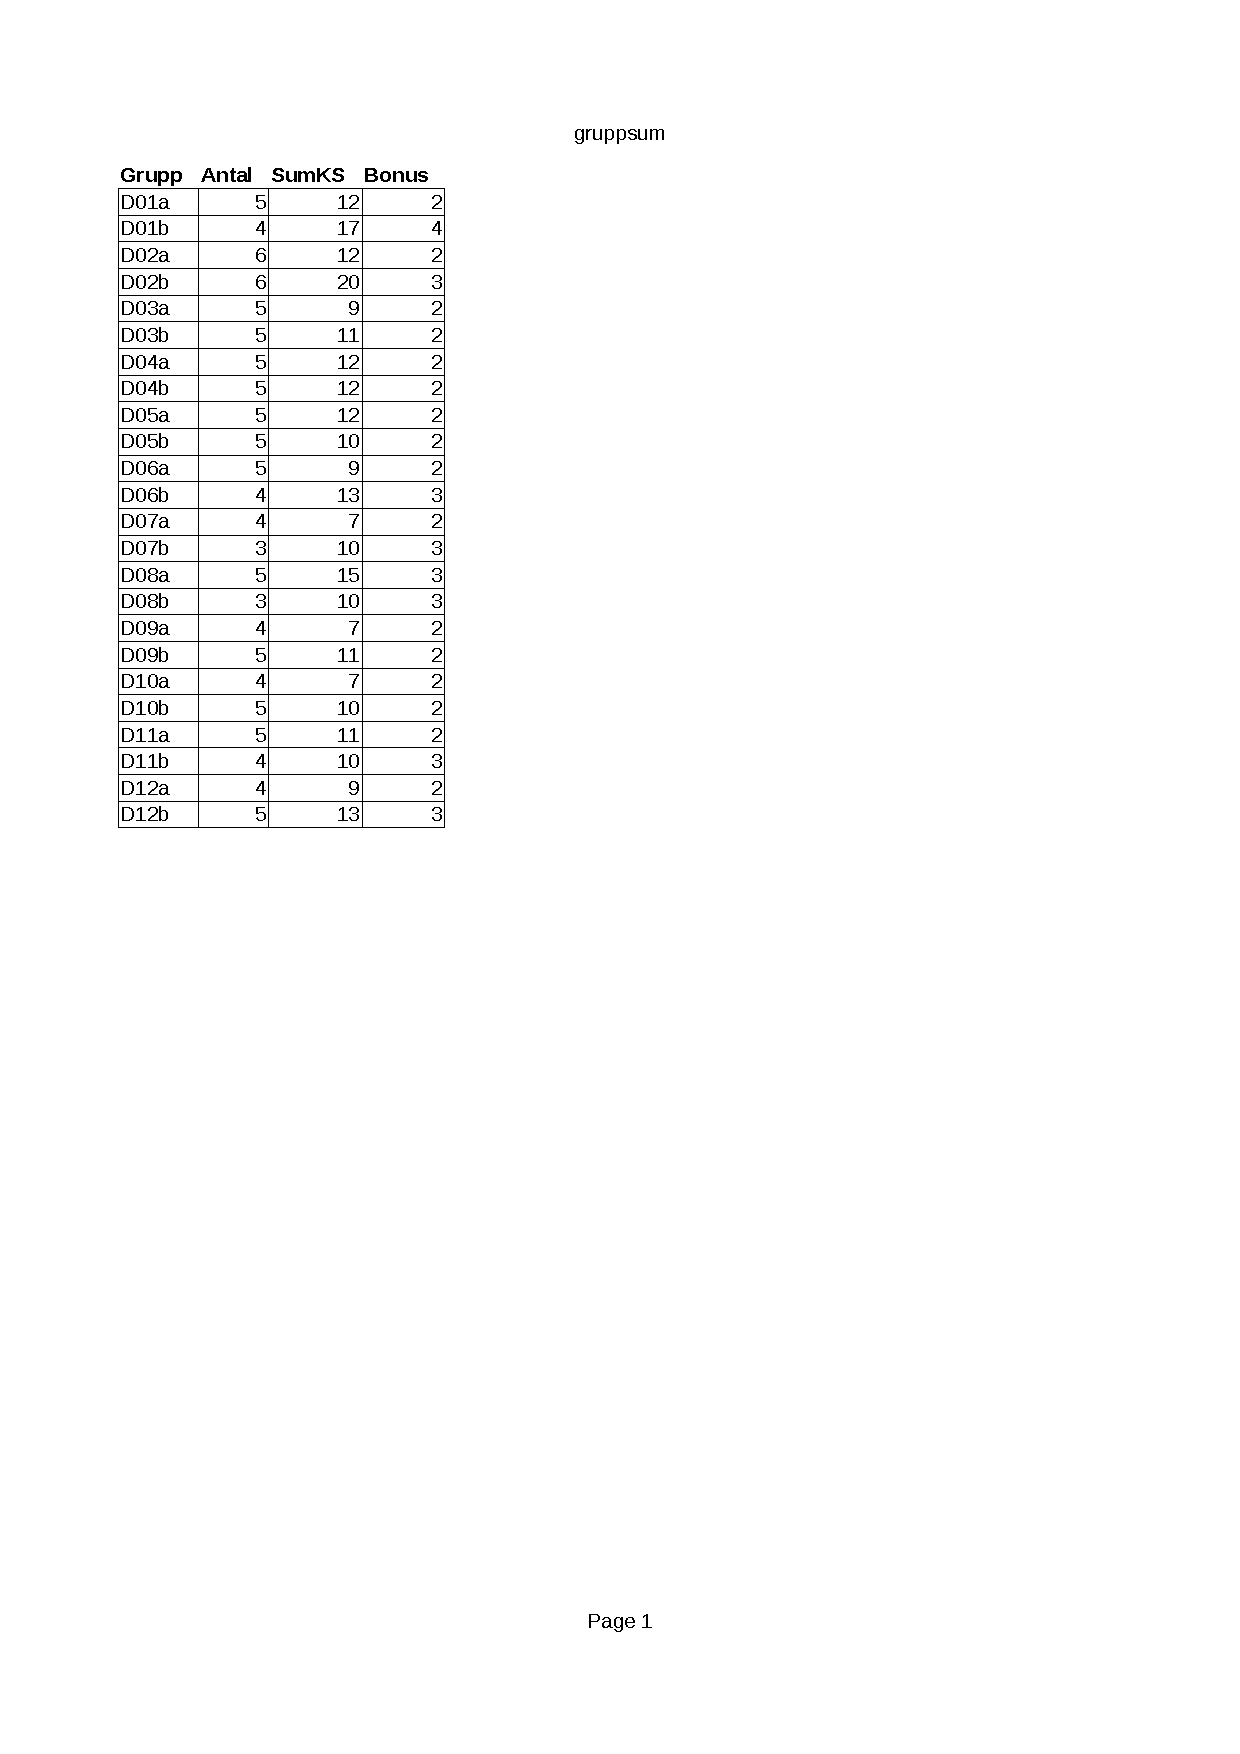
\includegraphics[clip, trim=0cm 1cm 3.2cm 2.5cm, width=0.9\textwidth]{../img/bonus-2016.pdf}

\columnbreak

\begin{itemize}
\pause
\item Bonus gäller vid första ordinarie tentatillfälle 
\pause
\item D07b och D08b har 3 st; \\ vill ni göra merge?

\end{itemize}
\end{multicols}
\end{Slide}

\Subsection{Specialundervisning}
\begin{Slide}{Specialundervisning}
Under vecka w09 och w10 (till att börja med) kommer vi att organisera \Emph{specialundervisning} under dessa \Alert{resurstider}:
\begin{itemize}
\item \Emph{Torsdag kl 8-10} i både \Alert{Falk} och \Alert{Val}  (Gustav, Valthor, Emil)
\item \Emph{Torsdag kl 10-12} i \Alert{Falk} (Maj)
\item OBS! Dessa rumtider är till för de som hade 0 eller 1 på kontrollskrivningen och som ansökt om specialundervisning via länk i speciell mejlinbjudan. 
\end{itemize}
\SlideFontSmall{Undantag: Om du har mer än 1 på kontrollskrivningen men inte alls har möjlighet att gå på någon annan resurstid än ovan är du också välkommen; anmäl då din situation till handledaren på plats och så får du vara med i gruppen och kan få svar på frågor etc. som vanligt.}
\end{Slide}
\fi












%!TEX encoding = UTF-8 Unicode
%!TEX root = ../lect-week09.tex

%%%


%\begin{Slide}{TODO: Begrepp att förklara}
%  Tänk igenom ordningen:
%  \begin{itemize}
%    \item java switch, scala match ... 
%  \end{itemize}
%\end{Slide}
%
%
%\begin{Slide}{Javas switch-sats}
%A switch in Java works with the byte, short, char, and int primitive data types. It also works with enumerated types (discussed in Enum Types), the String class, and a few special classes that wrap certain primitive types: Character, Byte, Short, and Integer
%\end{Slide}


\begin{Slide}{Javas switch-sats}

\begin{CodeSmall}[language=Java]
public class Switch {
    public static void main(String[] args) {
        String favorite = "selleri";
        if (args.length > 0) {
            favorite = args[0];
        }
        System.out.println("Din favoritgrönsak: " + favorite);
        char firstChar = Character.toLowerCase(favorite.charAt(0));
        System.out.print("Jag tycker ");
        switch (firstChar) {
        case 'g': 
            System.out.println("gurka är gott!");
            break;
        case 't': 
            System.out.println("tomat är gott!");
            break;
        case 'b': 
            System.out.println("brocolli är gott!");
            break;
        default:
            System.out.println(favorite + " är mindre gott...");
            break;
        }
    }
}
\end{CodeSmall}
\end{Slide}













%!TEX encoding = UTF-8 Unicode
%!TEX root = ../lect-week09.tex

%%%

\ifkompendium\else


\Subsection{Option}


\begin{Slide}{Hur hantera saknade värden?}\SlideFontSmall
Olika sätt att hantera saknade värden:
\begin{itemize}
\item Hitta på ett specialvärde: exempel -1 för icke nedtryckt sträng
\item \code{null} om \code{AnyRef}/\code{Object} (vanligt i Java, mkt ovanligt i Scala) 
\item Använd en samling och låt tom samling representera saknad värde: \\
\code{val grip = Vector(Vector(2), Vector(7), Vector(), Vector(3))}

\item \code{Option[T]} gemensam bastyp för: \\
  \code{None} som representerar \Alert{saknat värde}, och \\ \code{Some[T]} som representerar att \Emph{värde finns}
\end{itemize}
\end{Slide}

\begin{Slide}{En gemensam bastyp för ett värde som kanske saknas}\SlideFontSmall
\vspace{-0.5em}\begin{center}
\newcommand{\TextBox}[1]{\raisebox{0pt}[1em][0.5em]{#1}}
\tikzstyle{umlclass}=[rectangle, draw=black,  thick, anchor=north, text width=3cm, rectangle split, rectangle split parts = 3]
\begin{tikzpicture}[inner sep=0.5em]
\node [umlclass, rectangle split parts = 2, xshift=0cm, text width=3.5cm] (BaseType)  {
            \textit{\textbf{\centerline{\TextBox{\code{Option[A]}}}}}
            \nodepart[]{second}
            \TextBox{\code{def get: A}}\newline
            \TextBox{\code{def isEmpty: Boolean}}

        };
        
\node [umlclass, rectangle split parts = 1]  at (-2.5cm,-3.7cm) (SubType1) {
            \textbf{\centerline{\TextBox{\code{Some[A]}}}}
            % \nodepart[]{second} \TextBox{\code{val x: A}}
        };  
                
\node [umlclass, rectangle split parts = 1] at (2.5cm,-3.7cm) (SubType2)  {
            \textbf{\centerline{\TextBox{\code{None}}}}
        };        
\draw[umlarrow] (SubType1.north) -- ++(0,0.5) -| (BaseType.south);    
\draw[umlarrow] (SubType2.north) -- ++(0,0.5) -| (BaseType.south);            
\end{tikzpicture}
\end{center}
\end{Slide}


\begin{Slide}{Option för hantering av ev. saknade värden}\SlideFontSmall
Alla vill inte berätta för Facebook vad de har för kön. \\ Förbättra Facebooks kod med ett litet Scala-program:
\begin{Code}
trait Gender
case object Male   extends Gender
case object Female extends Gender

case class Person(name: String, gender: Option[Gender])
\end{Code}
\pause
\begin{REPL}
scala> val p1 = Person("Björn",  Some(Male))
scala> val p2 = Person("Sandra", Some(Female))
scala> val p3 = Person("Andro",  None)
scala> val g2 = p2.gender
scala> def show(g: Option[Gender]): String = g match {
         case Some(x) => x.toString
         case None    => "unknown"
       }
scala> show(g2)
scala> show(p3.gender)
scala> val ps = Vector(p1,p2,p3)
scala> ps.map(_.gender).map(show)
\end{REPL}
\end{Slide}

\begin{Slide}{Några smidiga metoder på \code{Option}}
getOrElse

map

foreach

isEmpty
\end{Slide}


\begin{Slide}{Några samlingsmetoder som ger en \code{Option}}
get på Map

headOption på Vector

find på Seq
\end{Slide}



\fi



%!TEX encoding = UTF-8 Unicode
%!TEX root = ../lect-week09.tex

%%%


\ifkompendium\else

\Subsection{Undantag}
\begin{Slide}{Vad är ett undantag \Eng{exception}?}
Undantag representerar ett fel eller ett onormalt tillstånd som upptäcks under exekvering och som  behöver hanteras på särskilt sätt vid sidan av det normala exekveringsflödet. 

\vspace{1em}\href{https://sv.wikipedia.org/wiki/Undantagshantering}{sv.wikipedia.org/wiki/Undantagshantering}


\vspace{1em} Exempel på undantag:

\pause

\begin{itemize}
\item Indexering utanför vektorns indexgränser.

\item Läsning bortom filens slut.

\item Försök att öppna en fil som inte finns.

\item Minnet är slut.

\item Division med noll.

\item \code{"hej".toInt} resulterar i \\\code{java.lang.NumberFormatException}

\end{itemize}

\end{Slide}

\begin{Slide}{''Kasta'' dina egna undantag med \texttt{throw}}\SlideFontSmall
Man kan själv generera ett undantag med \code{throw}, vilket kallas att \Emph{kasta} ett undantag som (om det inte \Emph{fångas}), gör att exekveringen \Alert{avbryts}.


\begin{REPL}
scala> def pang = throw new Exception("PANG!")
pang: Nothing

scala> pang
java.lang.Exception: PANG!
  at .pang(<console>:11)
  ...
  
\end{REPL}
\pause
Olika sätt att hantera undantag: 
\begin{itemize}
\item Scala: Man kan använda ett \code{try ... catch}-uttryck och ge ett \Emph{värde} i händelse av undantag.
\item Java: Man kan använda en \code{try ... catch}-sats och \Alert{göra något} i händelse av undantag.
 
\item Scala: Man kan \Emph{kapsla in} ett undantag med \Emph{\texttt{scala.util.Try}} och förhindra att exekveringen avbryts. (Finns ej i Java; att föredra i Scala.)
\end{itemize}
\end{Slide}


\Subsection{\texttt{scala.util.Try}}

\begin{Slide}{En gemensam bastyp för något som kan misslyckas}\SlideFontSmall
\begin{Code}
import scala.util.{Try, Success, Failure}
\end{Code}

\vspace{-0.5em}\begin{center}
\newcommand{\TextBox}[1]{\raisebox{0pt}[1em][0.5em]{#1}}
\tikzstyle{umlclass}=[rectangle, draw=black,  thick, anchor=north, text width=3.0cm, rectangle split, rectangle split parts = 3]
\begin{tikzpicture}[inner sep=0.5em]
\node [umlclass, rectangle split parts = 2, xshift=0cm, text width=3.8cm] (BaseType)  {
            \textit{\textbf{\centerline{\TextBox{\code{Try[T]}}}}}
            \nodepart[]{second}
            \TextBox{\code{def get: T}}\newline
            \TextBox{\code{def isFailure: Boolean}}\newline
            \TextBox{\code{def isSuccess: Boolean}}
        };
        
\node [umlclass, rectangle split parts = 2, text width=2.2cm]  at (-2.5cm,-3.7cm) (SubType1) {
            \textbf{\centerline{\TextBox{\code{Success[T]}}}}
            \nodepart[]{second} \TextBox{\code{val value: T}}
        };  
                
\node [umlclass, rectangle split parts = 2, text width=4.2cm] at (2.5cm,-3.7cm) (SubType2)  {
            \textbf{\centerline{\TextBox{\code{Failure[T]}}}}
            \nodepart[]{second} \TextBox{\code{val exception: Throwable}}
        };        
\draw[umlarrow] (SubType1.north) -- ++(0,0.5) -| (BaseType.south);    
\draw[umlarrow] (SubType2.north) -- ++(0,0.5) -| (BaseType.south);            
\end{tikzpicture}
\end{center}
\end{Slide}

\begin{Slide}{Hantera undantag med \texttt{Try}}
\vspace{-0.5em}\begin{REPL}
scala> def pang = throw new Exception("PANG!")

scala> def kanskePang = if (math.random < 0.5) 42 else pang

scala> import scala.util.{Try, Success, Failure}

scala> def försök = Try { kanskePang }

scala> val xs = Vector.fill(15){försök}

scala> val trettonde = xs(13) match {
         case Success(value) => value
         case Failure(e) => println(e); -1
       }

scala> (xs(13).isSuccess, xs(13).isFailure)

scala> försök.foreach(println)

scala> försök.map(_ + 1)

scala> for (Success(x) <- xs) yield x
\end{REPL}
\end{Slide}

\begin{Slide}{Fördjupning: \texttt{try}-\texttt{catch}-uttryck}\SlideFontSmall
Man kan fånga undantag med ett \code{try ... catch}-uttryck:
\begin{Code}
def carola = try {
  if (math.random > 0.5) throw new Exception("stormvind")
  42
} catch { 
  case e: Exception =>
    println("Fångad av en " + e.getMessage)
    -1
}  
\end{Code}
\pause
\begin{REPL}
scala> Vector.fill(5)(carola)
Fångad av en stormvind
Fångad av en stormvind
Fångad av en stormvind
res0: scala.collection.immutable.Vector[Int] = Vector(-1, 42, 42, -1, -1)
\end{REPL}
\pause
\emph{Fördjupning:} \\ Gör övning 9-10 som visar hur man fångar undantag i Scala och Java. \\Mer om undantag i fortsättningskursen.
\end{Slide}


\fi






%!TEX encoding = UTF-8 Unicode
%!TEX root = ../lect-week09.tex

%%%

\ifkompendium\else
\Subsection{Mer om \texttt{equals}}
\begin{Slide}{Fördjupning: Implementera \texttt{equals} med \texttt{match}}
Det visar sig att innehållslikhet är förvånansvärt komplicerat att implementera i samband med arv.
\begin{itemize}
\item Det enklare fallet: Gör övning \code{matching:12} och implementera \code{equals} för innehållslikhet utan arv. \\ En bra träning på att använda \code{match}!

\item Svårare: Gör fördjupningsövning \code{matching:19} om du vill se hur en \emph{komplett} \code{equals} ska se ut som funkar i alla lägen.

\end{itemize}

Det ingår inte på tentan att själv kunna implementera en genrellt fungerande \code{equals}. Men du ska förstå skillnaden mellan referenslikhet och innehållslikhet. Mer om \code{equals} i fortsättningkursen.
\end{Slide}
\fi












\end{document}






